\part{Lecture 14: Outlook and Research Insights}
\title[RL Lecture 14]{Lecture 14: Outlook and Research Insights}
\date{}  
\frame{\titlepage} 

%%%%%%%%%%%%%%%%%%%%%%%%%%%%%%%%%%%%%%%%%%%%%%%%%%%%%%%%%%%%%%%%%%
\section{Safe Reinforcement Learning} 
%%%%%%%%%%%%%%%%%%%%%%%%%%%%%%%%%%%%%%%%%%%%%%%%%%%%%%%%%%%%%%%%%%
\begin{frame}
\frametitle{Table of contents}
\tableofcontents[currentsection]
\end{frame}

%%%%%%%%%%%%%%%%%%%%%%%%%%%%%%%%%%%%%%%%%%%%%%%%%%%%%%%%%%%%%
%% Recap: optimal control and constraints %%
%%%%%%%%%%%%%%%%%%%%%%%%%%%%%%%%%%%%%%%%%%%%%%%%%%%%%%%%%%%%%
\frame{\frametitle{Recap: optimal control and constraints}
Real-world systems are always subject to certain state constraints $\mathcal{X}$ and input limitations $\mathcal{U}$. Violating those can lead to safety issues.   
\begin{equation}
	\begin{split}
	v_k^* &= \max_{\bm{u}_k} \sum_{i=0}^{N_\mathrm{p}} \gamma^i r_{k+i+1} (\bm{x}_{k+i}, \bm{u}_{k+i})\, ,\\
	\mathrm{s.t.} \quad\quad \bm{x}_{k+i+1}&=\bm{f}(\bm{x}_{k+i},\bm{u}_{k+i}), \quad \bm{x}_{k+i} \in \mathcal{X},\quad \bm{u}_{k+i} \in \mathcal{U}\,.\\
\end{split}
\end{equation}
\begin{figure}
\centering
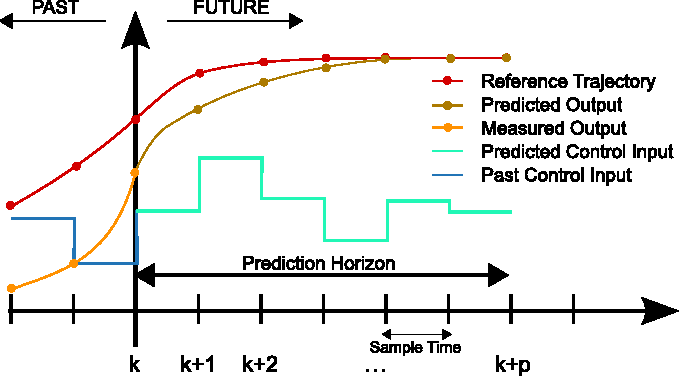
\includegraphics[height=0.4\textheight]{fig/lec01/MPC.pdf}
\caption{MPC scheme (source: \href{https://de.wikipedia.org/wiki/Model_Predictive_Control}{www.wikipedia.org},  by Martin Behrendt \href{https://creativecommons.org/licenses/by-sa/3.0/deed.en}{CC BY-SA 3.0})}
\label{fig:MPC}
\end{figure}
}

%%%%%%%%%%%%%%%%%%%%%%%%%%%%%%%%%%%%%%%%%%%%%%%%%%%%%%%%%%%%%
%% Application examples with safety concerns %%
%%%%%%%%%%%%%%%%%%%%%%%%%%%%%%%%%%%%%%%%%%%%%%%%%%%%%%%%%%%%%
\frame{\frametitle{Application examples with safety-relevant constraints}
\begin{figure}
 \centering
 \begin{columns}
        \column{.2\linewidth}
				\caption*{Collaborative robot control (source: \href{https://commons.wikimedia.org/wiki/File:Human-Robot-Collaboration-Sawing-2016-Luka-Peternel.jpg}{www.wikipedia.org}, \href{https://creativecommons.org/licenses/by-sa/4.0/deed.en}{CC BY-SA 4.0})}
        \column{.3\linewidth}
        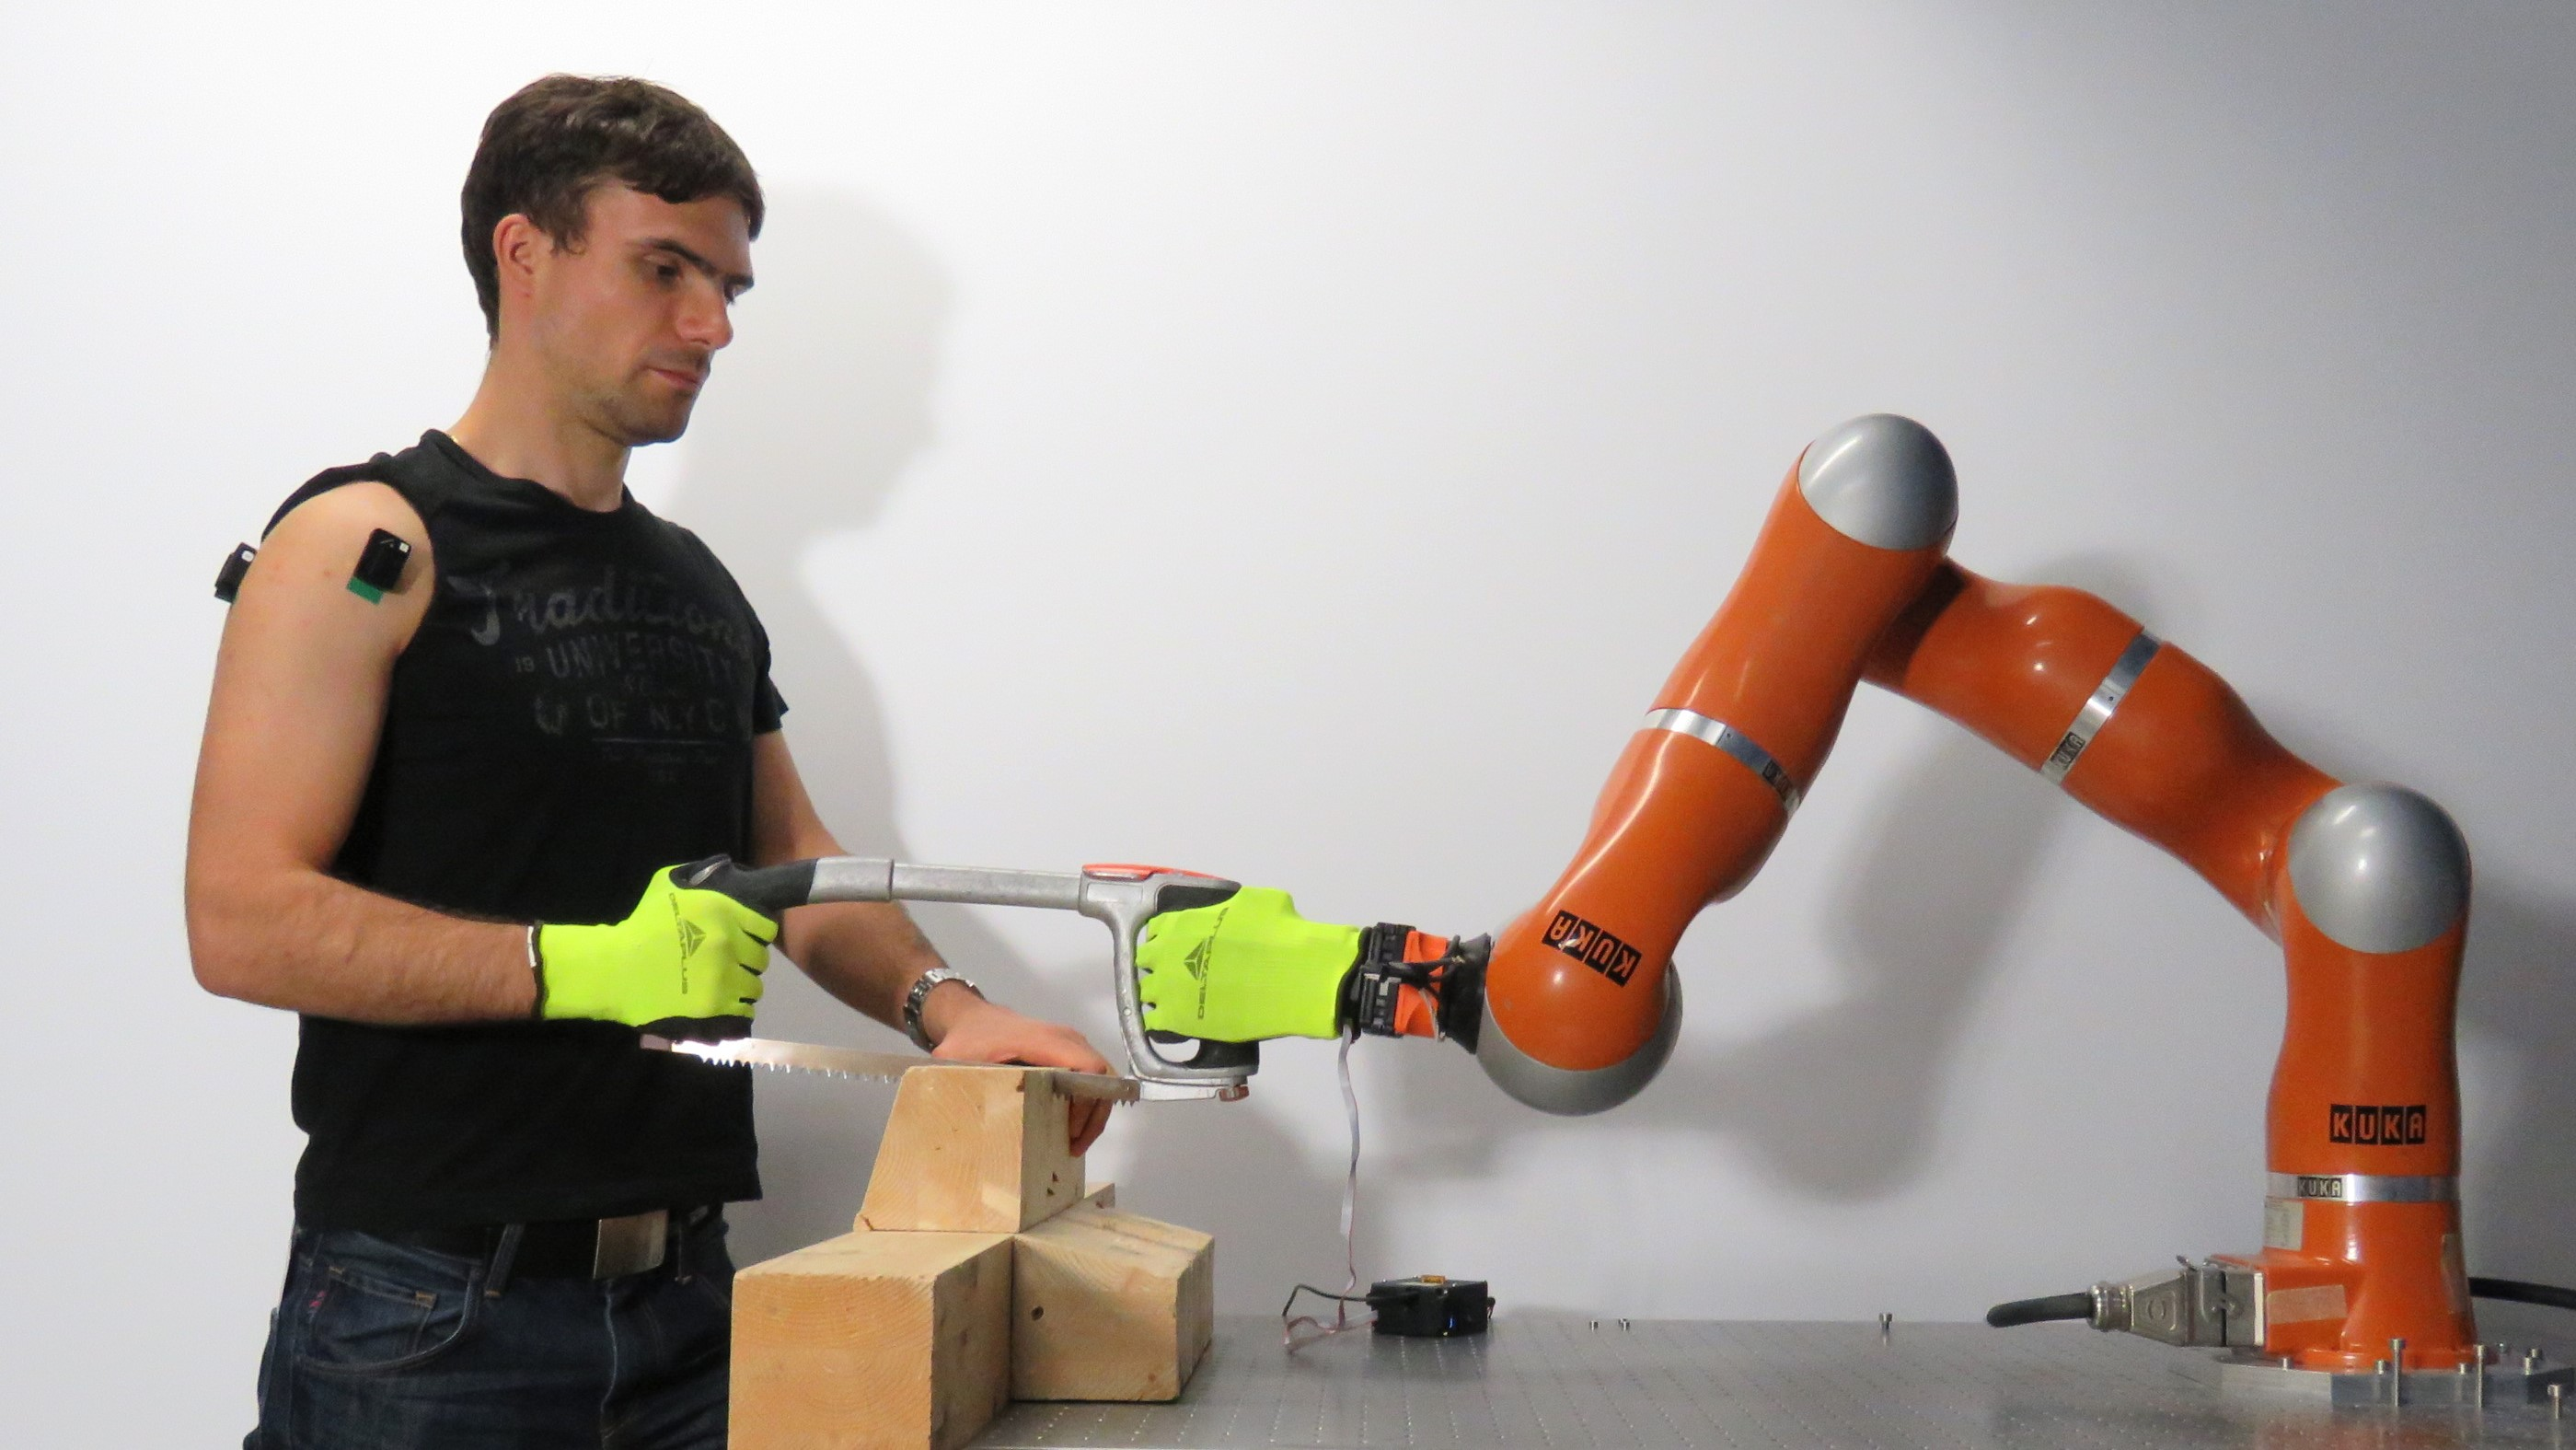
\includegraphics[width=\textwidth]{fig/lec14/Human-Robot-Collaboration.jpg}
				\column{.3\linewidth}
        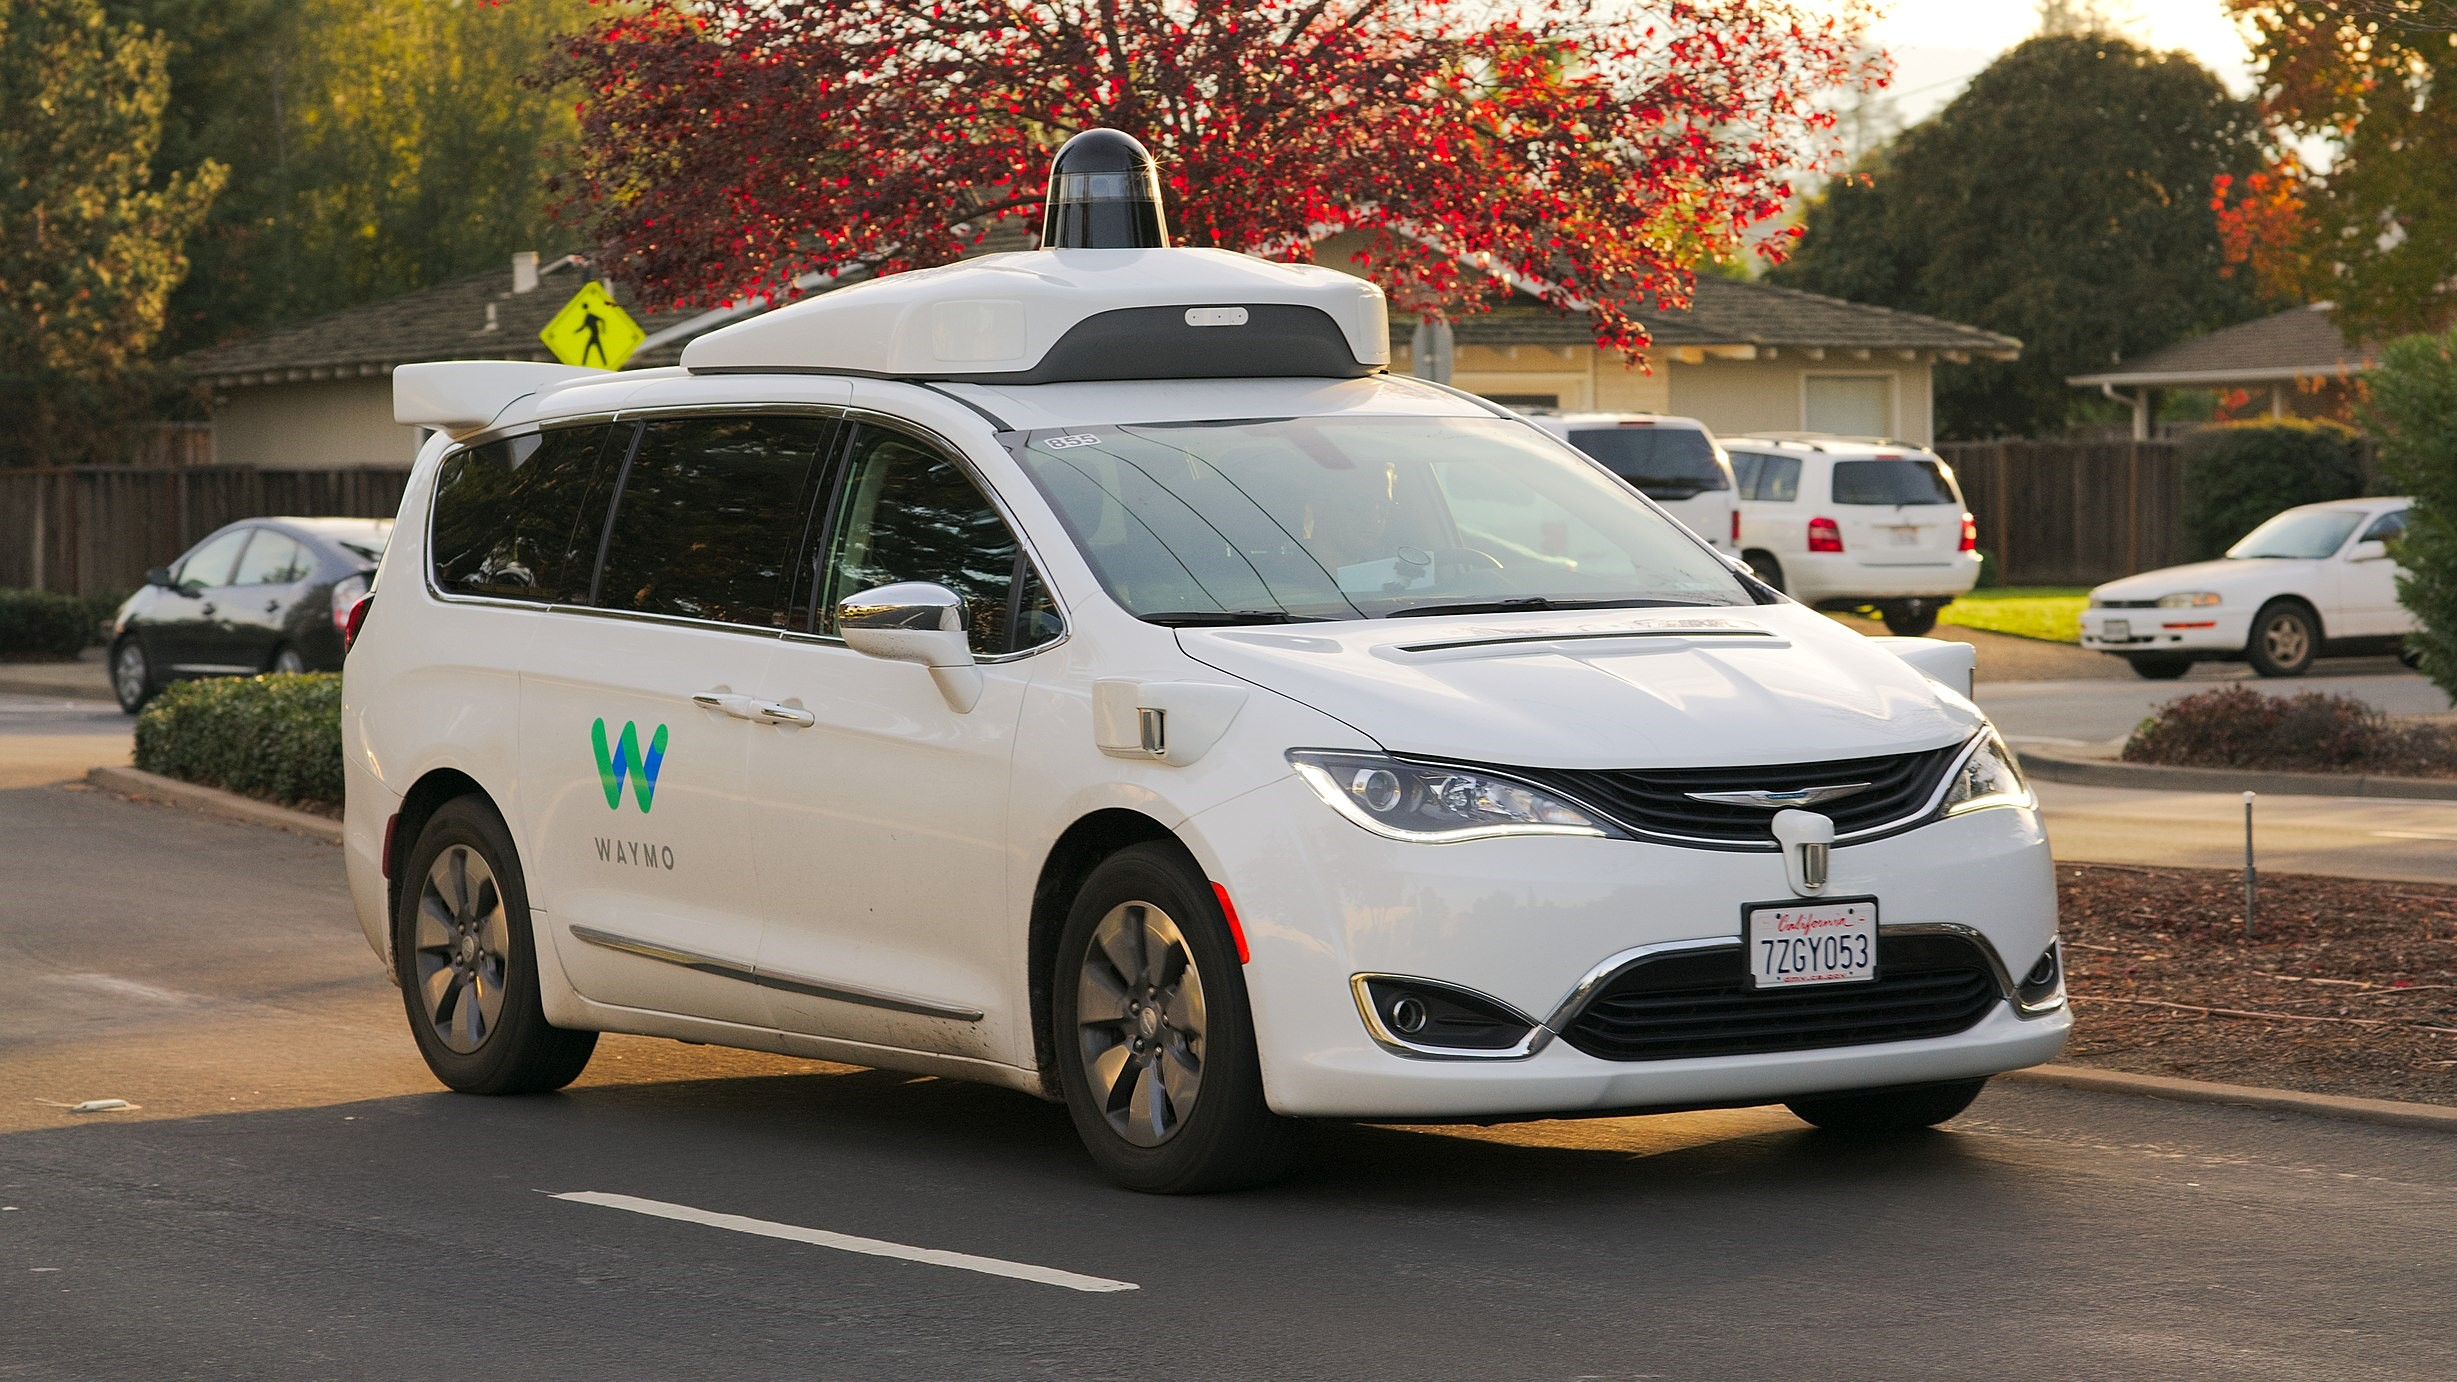
\includegraphics[width=\textwidth]{fig/lec14/Waymo.jpg}
				\column{.2\linewidth}
				\caption*{Autonomous car driving (source: \href{https://commons.wikimedia.org/wiki/File:Waymo_Chrysler_Pacifica_in_Los_Altos,_2017.jpg}{www.wikipedia.org}, \href{https://creativecommons.org/licenses/by-sa/4.0/deed.en}{CC BY-SA 4.0})}
      \end{columns}
			\vspace{1cm}
			\begin{columns}
        \column{.2\linewidth}
				\caption*{Energy system control}
        \column{.3\linewidth}
        \includegraphics[width=\textwidth]{fig/lec14/microgrid.jpg}
				\column{.3\linewidth}
        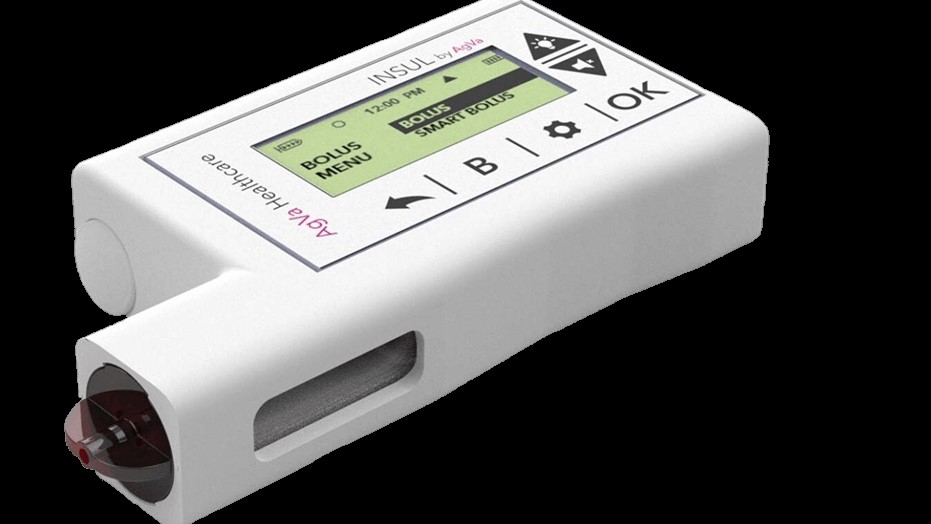
\includegraphics[width=\textwidth]{fig/lec14/Insulin_pump.jpg}
				\column{.2\linewidth}
				\caption*{Medication control (source: \href{https://commons.wikimedia.org/wiki/File:Insulin_pump.png}{www.wikipedia.org}, \href{https://creativecommons.org/licenses/by-sa/4.0/deed.en}{CC BY-SA 4.0})}
      \end{columns}
    \end{figure}
}

%%%%%%%%%%%%%%%%%%%%%%%%%%%%%%%%%%%%%%%%%%%%%%%%%%%%%%%%%%%%%
%% Safety levels %%
%%%%%%%%%%%%%%%%%%%%%%%%%%%%%%%%%%%%%%%%%%%%%%%%%%%%%%%%%%%%%
\frame{\frametitle{Safety levels}
\begin{figure}
\centering
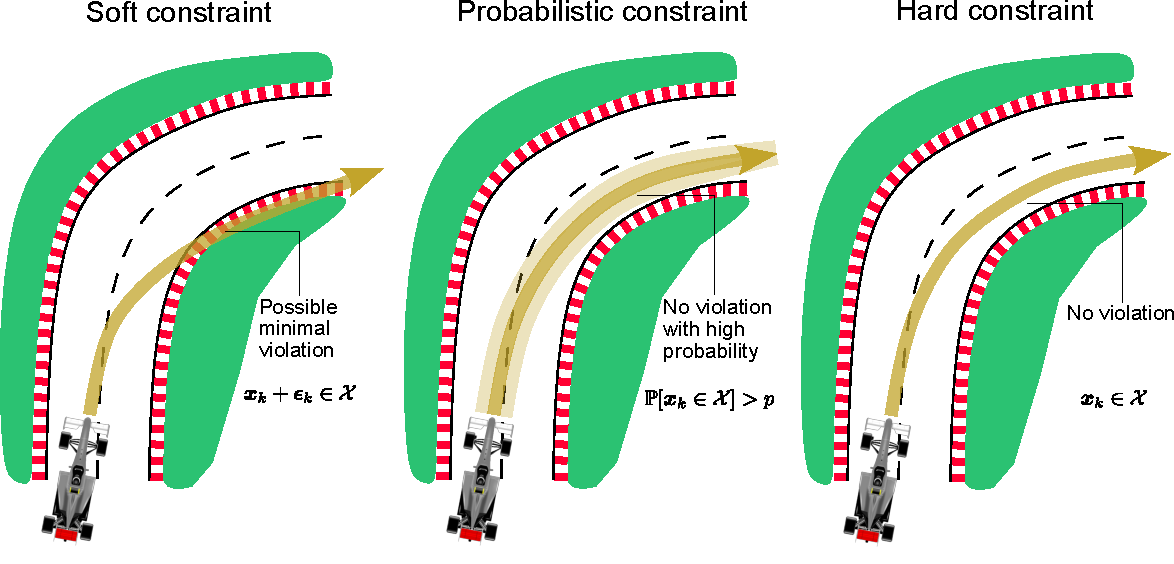
\includegraphics[height=0.68\textheight]{fig/lec14/Safety_Levels.pdf}
\caption{Different levels of safety (derived from L. Brunke et al., \textit{Safe Learning in Robotics: From Learning-Based Control to Safe Reinforcement Learning}, Annual Review of Control, Robotics, and Autonomous Systems, 2022)}
\label{fig:safety_levels}
\end{figure}
}

%%%%%%%%%%%%%%%%%%%%%%%%%%%%%%%%%%%%%%%%%%%%%%%%%%%%%%%%%%%%%
%% Bird's eye view on RL concepts integrating safety %%
%%%%%%%%%%%%%%%%%%%%%%%%%%%%%%%%%%%%%%%%%%%%%%%%%%%%%%%%%%%%%
\frame{\frametitle{Bird's eye view on RL concepts integrating safety}
\vspace{-0.1cm}
\begin{figure}%
\centering
\subfloat[][Safety critic: add a critic which indicates to which extent the current data sample fits to a safe situation]{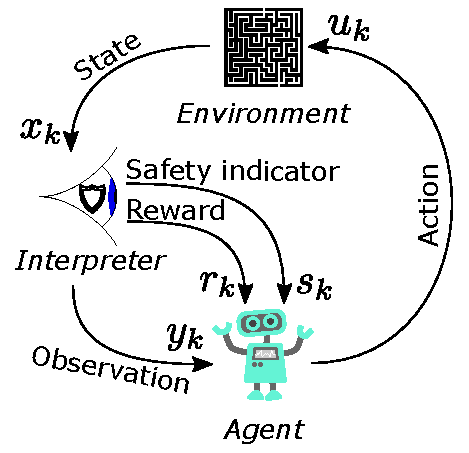
\includegraphics[width=0.375\textwidth]{fig/lec14/RL_Safety_Critic.pdf}}%
\qquad
\subfloat[][Safety shield: use a priori or learned model knowledge of the environment to make predictions identifying actions leading to unsafe situations]{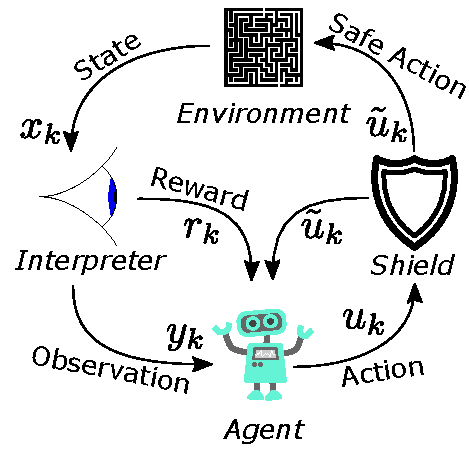
\includegraphics[width=0.375\textwidth]{fig/lec14/Safe_RL_Shield.pdf}}%
\caption{Safety methods}%
\label{fig:safety_birds_eye}%
\end{figure}
}

%%%%%%%%%%%%%%%%%%%%%%%%%%%%%%%%%%%%%%%%%%%%%%%%%%%%%%%%%%%%%
%% Bird's eye view on RL concepts integrating safety %%
%%%%%%%%%%%%%%%%%%%%%%%%%%%%%%%%%%%%%%%%%%%%%%%%%%%%%%%%%%%%%
\frame{\frametitle{Achievable safety levels and model knowledge}
\begin{figure}
\centering
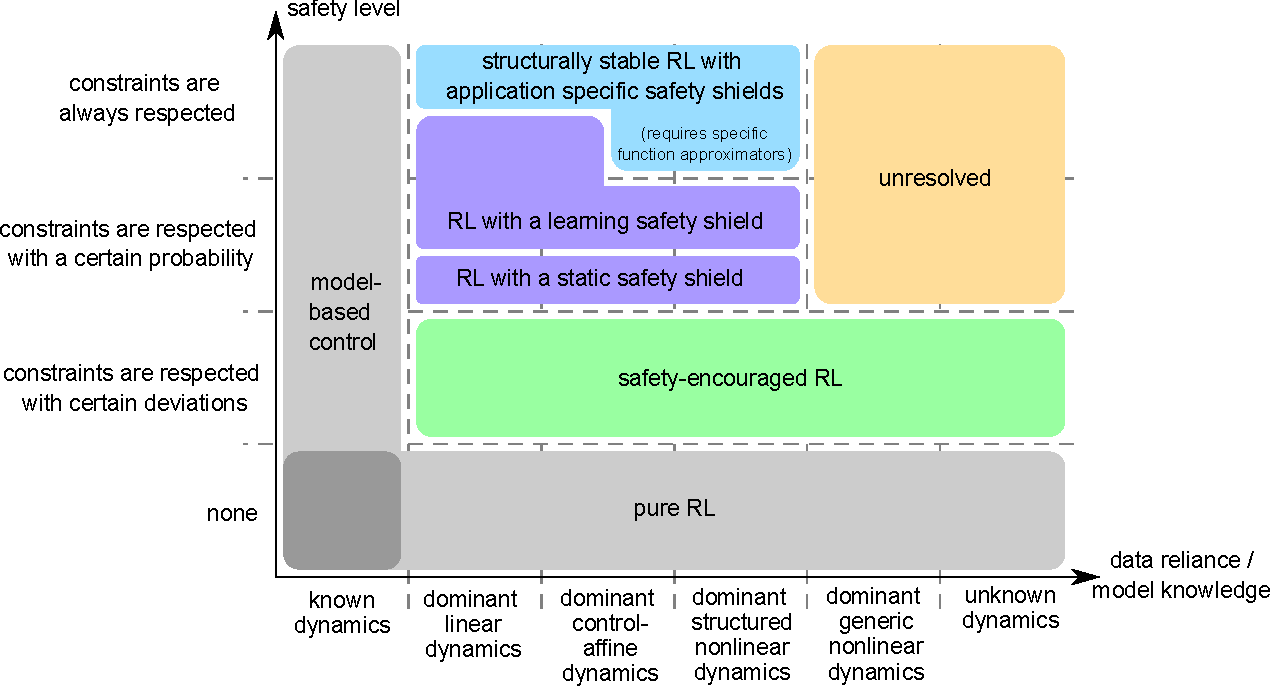
\includegraphics[height=0.68\textheight]{fig/lec14/Safeguard_Classes.pdf}
\caption{Safety and model knowledge map (derived from L. Brunke et al., \textit{Safe Learning in Robotics: From Learning-Based Control to Safe Reinforcement Learning}, Annual Review of Control, Robotics, and Autonomous Systems, 2022)}
\label{fig:safety_levels}
\end{figure}
}

%%%%%%%%%%%%%%%%%%%%%%%%%%%%%%%%%%%%%%%%%%%%%%%%%%%%%%%%%%%%%%%%%%
\section{Real-World Implementation with Fast Policy Inference} 
%%%%%%%%%%%%%%%%%%%%%%%%%%%%%%%%%%%%%%%%%%%%%%%%%%%%%%%%%%%%%%%%%%
\begin{frame}
\frametitle{Table of contents}
\tableofcontents[currentsection]
\end{frame}

%%%%%%%%%%%%%%%%%%%%%%%%%%%%%%%%%%%%%%%%%%%%%%%%%%%%%%%%%%%%%%%%%%
\section{Meta Reinforcement Learning} 
%%%%%%%%%%%%%%%%%%%%%%%%%%%%%%%%%%%%%%%%%%%%%%%%%%%%%%%%%%%%%%%%%%
\begin{frame}
\frametitle{Table of contents}
\tableofcontents[currentsection]
\end{frame}
